
%(BEGIN_QUESTION)
% Copyright 2010, Tony R. Kuphaldt, released under the Creative Commons Attribution License (v 1.0)
% This means you may do almost anything with this work of mine, so long as you give me proper credit

This diagram shows a sample system for a set of CEMS analyzers:

$$\includegraphics[width=15.5cm]{i02323x01.eps}$$

Identify and explain the consequence of a technician accidently leaving hand valve \#5 (V5) shut.  Assume everything else in this analyzer system is operating as it should.

\vskip 50pt

Identify and explain the consequence of the condensate pump failing (shutting off), being as specific as you can.  Assume everything else in this analyzer system is operating as it should.  

\vskip 50pt

\underbar{file i02323}
%(END_QUESTION)





%(BEGIN_ANSWER)

Identify and explain the consequence of a technician accidently leaving hand valve \#5 (V5) shut.  Assume everything else in this analyzer system is operating as it should.  {\bf All three analyzers will continue to receive stack gas while they are supposed to self-calibrate.  As a result, they will all ``fail'' their self-calibration checks.}

\vskip 10pt

Identify and explain the consequence of the condensate pump failing (shutting off), being as specific as you can.  Assume everything else in this analyzer system is operating as it should.  {\bf Condensed water will accumulate in the sump until it floods the sample pump and eventually all the analyzers.  The result will initially be stagnant indications, then thousands of dollars worth of ruined analyzers!}

\vskip 10pt

I recommend granting half-credit for each correct explanation (5 points each).

%(END_ANSWER)





%(BEGIN_NOTES)

{\bf This question is intended for exams only and not worksheets!}.

%(END_NOTES)

